%----------------------------------------------------------------
%
%  File    :  curriculumvitae-main.tex
%
%  Authors :  Philipp Schunker
% 
%  Created :  28 Jun 2019
% 
%  Changed :  28 Jun 2019
% 
%----------------------------------------------------------------

\thispagestyle{empty}
%\chapter{Lebenslauf Philipp Schunker}

\begin{comment}
\begin{figure}[htbp]
	%\centering
	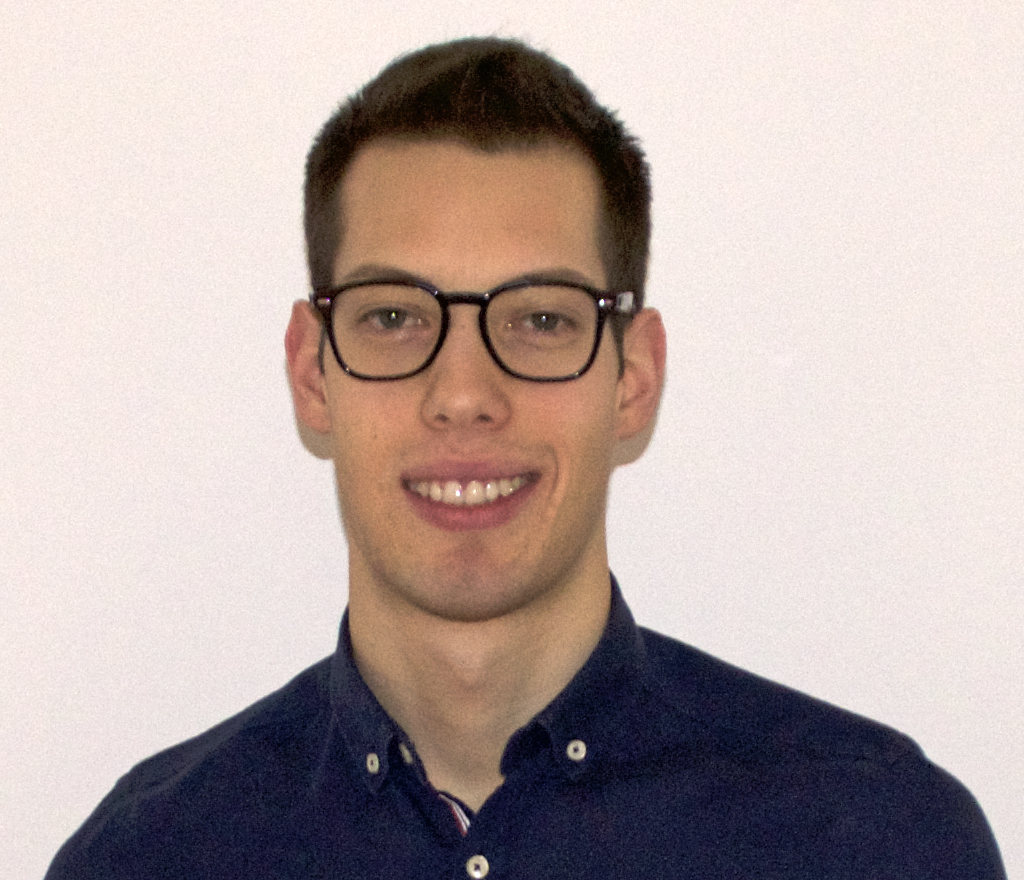
\includegraphics[height=5cm]{images/philipp}
\end{figure}
\end{comment}

\begin{minipage}{0.7\textwidth}
%Lebenslauf\\
\begin{addmargin}[2em]{2em}% 1em left, 2em right
\Large{\textbf{Lebenslauf}}\vspace{0.1cm}\\
\Large{\textbf{Philipp Schunker}}\vspace{1.0cm}\\
%\small{philipp@schunker.at}\vspace{0.5cm}\\
\end{addmargin}
\end{minipage}
\begin{minipage}{0.3\textwidth}
%\begin{figure}[htbp]
	%\centering
	 %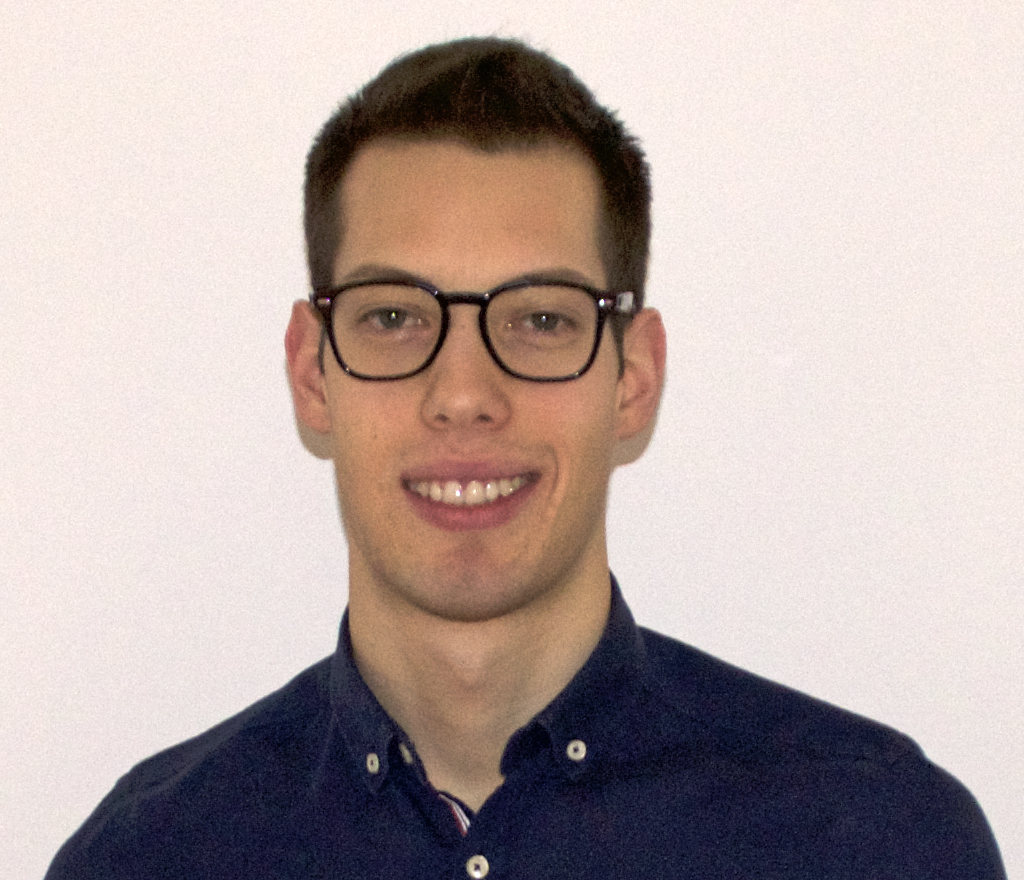
\includegraphics[width=0.6\textwidth]{images/philipp}
	 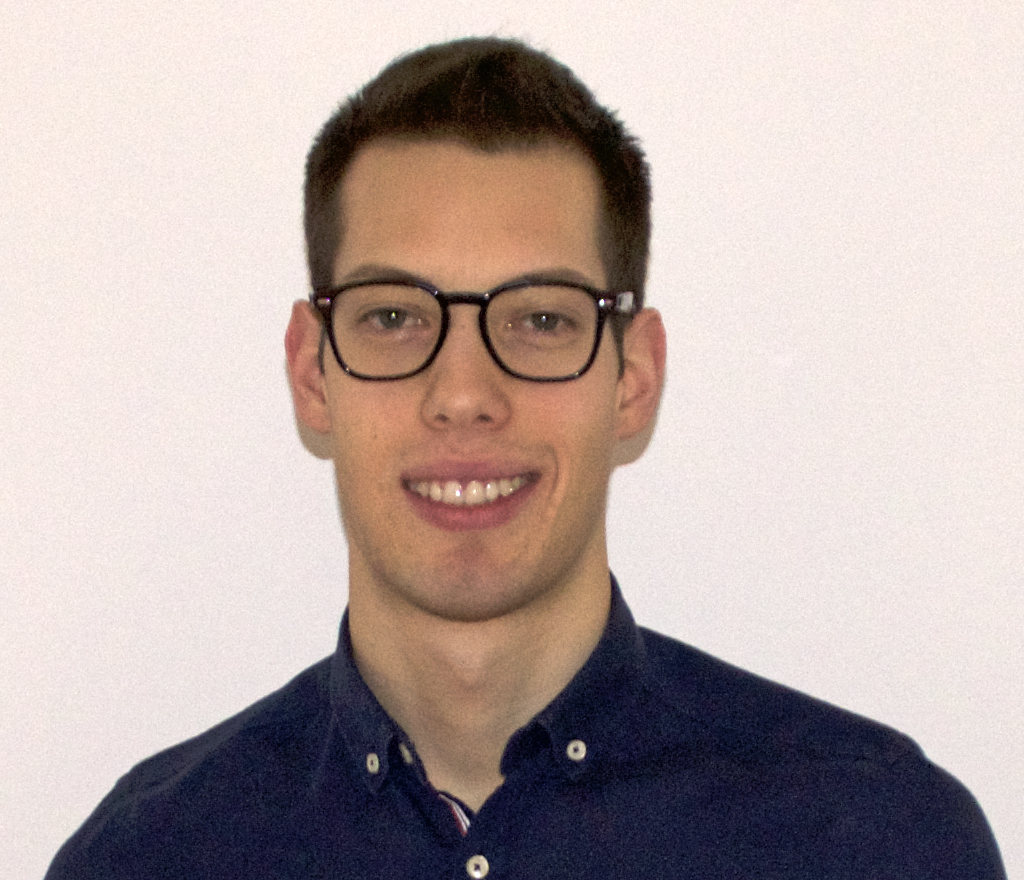
\includegraphics[width=\textwidth]{images/philipp}
%\end{figure}
\end{minipage}

\begin{comment}
\begin{table*}[htbp]
	\centering
		\begin{tabular}{|l|c|r|}
		%\hline
		%\rowcolor[gray]{0.9}
		%Spalte 1 & Spalte 2 & Spalte 3 \\
		\hline
		Affen & Giraffen & Löwen \\
		Äpfel & Birnen & Bananen \\
		Irgend & et & was \\
		\hline
		\end{tabular}
\end{table*}
\end{comment}

\begin{comment}
\begin{tabular*}{\textwidth}{c @{\extracolsep{\fill}} ccccc}
		\hline
		Affen & Giraffen & Löwen \\
		Äpfel & Birnen & Bananen \\
		Irgend & et & was \\
		\hline
\end{tabular*}
\end{comment}

\begin{comment}
\begin{longtabu} to \textwidth {l >{\bfseries}X[r, 2] X[4] l}
	\tableHeaderStyle
	& Angaben zur Person & & \\
        & Vorname Nachname & Philipp Schunker & \\
        & Staatsangehörigkeit & Österreich & \\
        & Geburtsdatum & 18.09.1991 & \\
        & Geschlecht & Männlich & \\
        	\tableHeaderStyle
	& Gewünschtes Berufsfeld & Leitender Software-Entwickler und Software-Architekt &\\
	\tableHeaderStyle
	& Berufserfahrung & & \\
	& Datum & November 2013 bis heute & \\
        & Funktion & IT Systems Engineer & \\
        & Arbeitgeber & Allianz Technology GmbH & \\
        & Tätigkeitsbereich & IT Operations - Application and System Services & \\ \bottomrule
        %----
        	& Datum & Juni 2013 bis Oktober 2013 & \\
        & Funktion & Junior Software Developer & \\
        & Arbeitgeber & Österreichisches Bundesheer, Führungsunterstützungzentrum Abteilung FüUZ/Applikation & \\
        & Tätigkeitsbereich & Applikationsentwicklung Intranet & \\ \bottomrule
        %----
        	& Datum & November 2011 bis Mai 2012 & \\
        & Funktion & Programmierer im Präsenzdienst & \\
        & Arbeitgeber & Österreichisches Bundesheer, Führungsunterstützungzentrum Abteilung FüUZ/Applikation & \\
        & Tätigkeitsbereich & Automatisierung der Qualitätssicherung von Webapplikationen & \\\bottomrule
        %----
        	& Datum & August 2010 bis September 2010 & \\
        & Funktion & Urlaubsaushilfe & \\
        & Arbeitgeber & Österreichische Post AG, Zustellbasis 1140 Wien & \\
        & Tätigkeitsbereich & Post-Zusteller & \\ \bottomrule
        %----
        	& Datum & Juli 2009 bis August 2009 & \\
        & Funktion & Berufspraktikum & \\
        & Arbeitgeber & 
        \begin{itemize}
	\item Service, Wartung und Instandsetzung von Computerhardware
	\item Entwicklung und Betreuung der intern genutzten Software und IT-Infrastruktur
	\end{itemize} & \\
        & Tätigkeitsbereich & Post-Zusteller & \\ \bottomrule
\end{longtabu}
\end{comment}

\begin{longtable}{p{0.3\textwidth}|p{0.7\textwidth}}%{r|l}
%\begin{longtabu} to \textwidth {>{\bfseries}X[r, 2] X[4]} %rl
%\begin{longtblr}
	%\tableHeaderStyle{Angaben zur Person} & \\
	\large{Angaben zur Person} & \\
	Vorname Nachname & Philipp Schunker \\
	Staatsangehörigkeit & Österreich \\
	Geburtsdatum & 18.09.1991 \\
	Geschlecht & Männlich \\
	E-Mail & philipp@schunker.at \\
	Telefonnummer & +43 699 1946 7200 \\
	Gewünschtes Berufsfeld & Leitender Software-Entwickler und Software-Architekt \\
	\bottomrule
	%\tableHeaderStyle
	%\large{Berufserfahrung} & \\
	\large{Berufserfahrung} & \\
	Datum & November 2013 bis heute \\
	Funktion & IT Systems/DevOps Engineer \\
	Arbeitgeber & Allianz Technology GmbH \\
	Tätigkeitsbereich & IT Operations - Application and System Services \\ \bottomrule
	%----
	Datum & September 2018 bis heute \\
	Funktion & Frei- und nebenberuflicher Software- und App-Entwickler \\
	Tätigkeitsbereich & Software-Entwicklung \\
	%& \small{\url{https://apps.apple.com/us/developer/philipp-schunker/id1437456240}} \\
	% & \begin{tabular}{cc}
	Veröffentlichungen, Produkte \& Dienste &
	\begin{comment}
	\begin{tabular}{m{.2\textwidth} m{.2\textwidth} }
	%\begin{itemize}[nosep,leftmargin=1em]
	%\item MapReminder
	%\end{itemize}
	MapReminder & 
\includegraphics[height=1.0cm]{images/iOS-MapReminder-1024} \\
	\end{tabular} \\
	& MapReminder ist eine leicht zu bedienende und im App Store verfügbare iOS App für ortsbezogene Erinnerungen \\
	& Diverse Open Source Software-Projekte auf GitHub \\
	\end{comment}
	\begin{tabular}{m{0.4\textwidth} m{0.02\textwidth} }
	\begin{itemize}[nosep,leftmargin=1em]
		\item MapReminder \newline
		%MapReminder ist eine leicht zu bedienende und im App Store verfügbare iOS App für ortsbezogene Erinnerungen
		MapReminder is an easy-to-use iOS App for location-based reminders available on the App Store
	\end{itemize}
	& 
\includegraphics[height=1.0cm]{images/iOS-MapReminder-1024} \\
	\begin{itemize}[nosep,leftmargin=1em]
		\item LoadMeter \newline
		%LoadMeter ist ein im Mac App Store verfügbares Dienstprogramm für die Anzeige der Systemauslastung
		LoadMeter is a utility program available on the Mac App Store for displaying the system load
	\end{itemize}
	& 
\includegraphics[height=1.0cm]{images/LoadMeter-1024-v2} \\
	\begin{itemize}[nosep,leftmargin=1em]
		\item Open Source Software-Projekte auf GitHub \newline
		\small{\url{https://github.com/philsch91}}
	\end{itemize}
	\end{tabular} \\
	\bottomrule
	%----
	Datum & Juni 2013 bis Oktober 2013 \\
	Funktion & Junior Software Developer \\
	Arbeitgeber & Österreichisches Bundesheer, Führungsunterstützungzentrum Abteilung FüUZ/Applikation \\
	Tätigkeitsbereich & Applikationsentwicklung Intranet \\
	\bottomrule
	\newpage
    %----
	Datum & November 2011 bis Mai 2012 \\
	Funktion & Programmierer im Präsenzdienst \\
	Arbeitgeber & Österreichisches Bundesheer, Führungsunterstützungzentrum Abteilung FüUZ/Applikation \\
	Tätigkeitsbereich & Automatisierung der Qualitätssicherung von Webapplikationen \\ \bottomrule
	%\newpage
	%----
	Datum & August 2010 bis September 2010 \\
	Funktion & Urlaubsaushilfe \\
	Arbeitgeber & Österreichische Post AG, Zustellbasis 1140 Wien \\
	Tätigkeitsbereich & Post-Zusteller \\ \bottomrule
	%\newpage
    %----
	Datum & Juli 2009 bis August 2009 \\
	Funktion & Berufspraktikum \\
	Arbeitgeber & Audio Video Media Service GmbH \\
	Tätigkeiten und Zuständigkeiten &
	%\tabitem Service, Wartung und Instandsetzung von Computerhardware \newline
	%Service, Wartung und Instandsetzung von Computerhardware \newline
	%\hangbullet{Entwicklung und Betreuung der intern genutzten Software und IT-Infrastruktur} \\
	%Entwicklung und Betreuung der intern genutzten Software und IT-Infrastruktur \\
	%\compress
	\begin{tabular} {m{.4\textwidth} m{0.05\textwidth} }
	\begin{itemize}[nosep,leftmargin=1em] 
	\item Service, Wartung und Instandsetzung von Computerhardware
    \item Entwicklung und Betreuung der intern genutzten Software und IT-Infrastruktur
	\end{itemize}
	\end{tabular}
	\\
	Tätigkeitsbereich & Informations- und Kommunikationstechnik \\
	\bottomrule
    %----
	Datum & Juli 2007 bis August 2007 \\
	Funktion & Berufspraktikum \\
	Arbeitgeber & Audio Video Media Service GmbH \\
	Tätigkeiten und Zuständigkeiten &
	%\tabitem Service, Wartung und Instandsetzung von Computerhardware \newline
	%\textbullet{Entwicklung und Betreuung der intern genutzten Software und IT-Infrastruktur} \\
	%\compress
	\begin{tabular} {m{.4\textwidth} m{0.05\textwidth} }
	\begin{itemize}[nosep,leftmargin=1em]
	\item Service, Wartung und Instandsetzung von Computerhardware
	\item Entwicklung und Betreuung der intern genutzten Software und IT-Infrastruktur
	\end{itemize}
	\end{tabular}
	\\
	Tätigkeitsbereich & Informations- und Kommunikationstechnik \\ \bottomrule
	%\tableHeaderStyle
	\large{Schul- und Berufsausbildung} & \\
	%----
	Datum & September 2019 bis Juli 2024 \\
	Name und Art der Bildungs- oder Ausbildungseinrichtung & University of Applied Sciences FH Campus Wien \newline
	Master Studiengang Software Design and Engineering \\
	Bezeichnung der erworbenen Qualifikation & Master of Science in Engineering (MSc) \\
	Publikationen &
	\begin{tabular} {m{.4\textwidth} m{0.05\textwidth} }
	\begin{itemize}[nosep,leftmargin=1em]
	\item Masterarbeit: Analysis on Decentralized Applications based on Ethereum
	\end{itemize}
	\end{tabular}
	\\
	Projekte \& Arbeiten & %\\
	\begin{tabular}{m{0.4\textwidth} m{0.02\textwidth} }
	%\begin{itemize}[nosep,leftmargin=0.5em,topsep=10pt]
	\begin{itemize}[nosep,leftmargin=1em]
	\item SpreadUtils \newline
	Software-Library für Group Communication basierend auf dem Spread toolkit in Java im Rahmen der Lehrveranstaltung \dq Dependable and Scalable Systems\dq
	\item CarRental \newline
	Software-Projekt für die praktische Umsetzung eines Software-Dienstes zur Miete von Straßenfahrzeugen für die Lehrveranstaltung \dq Service Engineering\dq. Microservice-Architektur, Backend-Komponenten in Java mit Spring Cloud, Spring Data JPA, H2 Database, MongoDB, RabbitMQ, Frontend-App für iOS in Swift mit UIKit.
	\end{itemize}
	\end{tabular} \\
	\bottomrule
	Datum & September 2016 bis September 2019 \\
	Name und Art der Bildungs- oder Ausbildungseinrichtung & University of Applied Sciences FH Campus Wien \newline
	Bachelorstudiengang Informationstechnologie und Telekommunikationstechnik \\
	Bezeichnung der erworbenen Qualifikation & Bachelor of Science in Engineering (BSc) \\
	Publikationen &
	\begin{tabular} {m{.4\textwidth} m{0.05\textwidth} }
	\begin{itemize}[nosep,leftmargin=1em]
	\item Bachelorarbeit 1: Pfadsuche basierend auf Reinforcement Learning und Monte-Carlo Tree Search
	\item Bachelorarbeit 2: Entscheidungsfindung basierend auf der Monte-Carlo Tree Search und künstlichen neuronalen Netzen
	\item Telekommunikation: Car-to-Car Communication
	%\scriptsize{\url{https://schunker-my.sharepoint.com/personal/philipp_schunker_at/_layouts/15/onedrive.aspx?id=\%2Fpersonal\%2Fphilipp\%5Fschunker\%5Fat\%2FDocuments\%2FAnlagen\%2FCar2CarCommuncation\%2Epdf&parent=\%2Fpersonal\%2Fphilipp\%5Fschunker\%5Fat\%2FDocuments\%2FAnlagen}}
	\item Internationalisierung@Home: What programming and logic have in common and how to write error-free software
	%\scriptsize{\url{https://schunker-my.sharepoint.com/personal/philipp_schunker_at/_layouts/15/onedrive.aspx?id=\%2Fpersonal\%2Fphilipp\%5Fschunker\%5Fat\%2FDocuments\%2FAnlagen\%2FFunctionalProgramming\%2Epdf&parent=\%2Fpersonal\%2Fphilipp\%5Fschunker\%5Fat\%2FDocuments\%2FAnlagen}}
	\end{itemize}
	\end{tabular}
	\\
	%\newpage
	Projekte \& Arbeiten & %\\
	\begin{tabular}{m{0.4\textwidth} m{0.02\textwidth} }
	%\begin{itemize}[nosep,leftmargin=0.5em,topsep=10pt]
	\begin{itemize}[nosep,leftmargin=1em]
	\item VienNav (MTCSNav) \newline
	Praktische Umsetzung für die Verifizierung und Auswertung der in der Bachelorarbeit 1 dargelegten Theorie
	\end{itemize}
	& 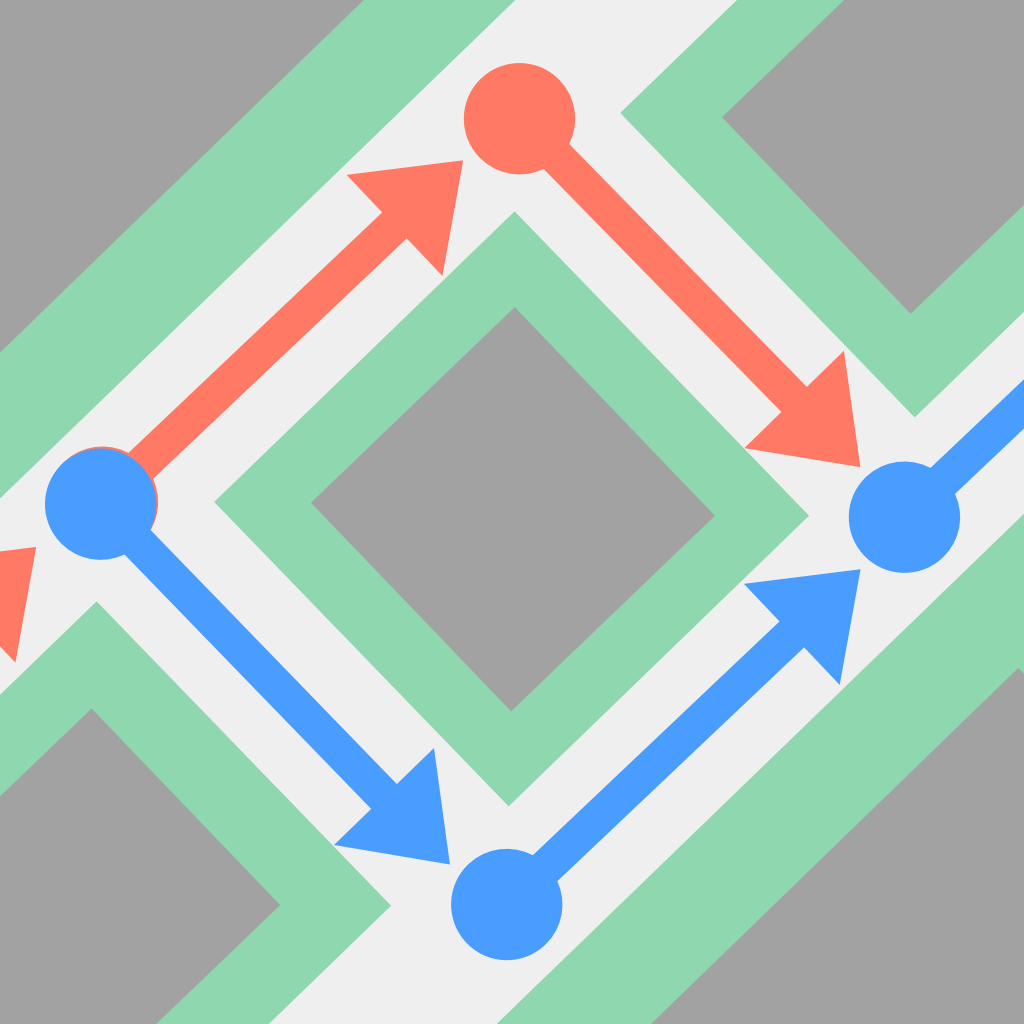
\includegraphics[height=1.0cm]{images/MCTS-Icon-1024} \\
	\begin{itemize}[nosep,leftmargin=1em]
	\item MLChess \newline
	Praktische Umsetzung für die Verifizierung und Auswertung der in der Bachelorarbeit 2 dargelegten Theorie
	\end{itemize}
 	& 
\includegraphics[height=1.0cm]{images/MLChess-Icon-1024} \\
	\end{tabular} \\
	%& Praktische Umsetzung für die Verifizierung und Auswertung der in der Bachelorarbeit 1 dargelegten Theorie \\
	\bottomrule
	%\newpage
    %----
    Datum & Oktober 2012 bis Mai 2013 \\
    Name und Art der Bildungs- oder Ausbildungseinrichtung & FH des bfi Wien Bachelorstudiengang Projektmanagement und IT \\ \bottomrule
    %----
    Datum & September 2006 bis Juni 2011 \\
    %Name und Art der Bildungs- oder Ausbildungseinrichtung & Höhere Technische Bundeslehranstalt Wien 16 \\
	Name und Art der Bildungs- oder Ausbildungseinrichtung & Höhere Technische Bundeslehranstalt Wien 16 \newline
	Informationstechnologie \newline mit Schwerpunkt Netzwerktechnik\\
    Bezeichnung der erworbenen Qualifikation & Diplom- und Reifeprüfung \\
    \bottomrule
    %Bezeichnung der Qualifikation & Abteilung Informationstechnologie mit Schwerpunkt Netzwerktechnik \\ 
    %\bottomrule
    %----
    Datum & September 2002 bis Juli 2006 \\
    Name und Art der Bildungs- oder Ausbildungseinrichtung & Bundesrealgymnasium Wien 8 Albertgasse Unterstufe \\ \bottomrule
    %----
    Datum & September 1998 bis Juli 2002 \\
    Name und Art der Bildungs- oder Ausbildungseinrichtung & Volksschule Wien 16 Grubergasse \\ 	\bottomrule
    %----
    Muttersprache & Deutsch \\
	Sonstige Sprache(n) & Englisch \\ %\bottomrule
	Selbstbeurteilung Englisch &
	%\begin{tabular}{| c | c | c | }
	\begin{tabular}{| c | c | c | c | c | c |}
	\hline
	%Verstehen & Sprechen & Schreiben \\
	%B2 & B2 & B2 \\
	\multicolumn{2}{| c |}{Verstehen} & \multicolumn{2}{| c |}{Sprechen} & \multicolumn{2}{| c |}{Schreiben} \\
	\hline
	Hören & Lesen & \multicolumn{2}{| c |}{} & \multicolumn{2}{| c |}{} \\
	\hline
	\multicolumn{2}{| c |}{C1} & \multicolumn{2}{| c |}{B2} & \multicolumn{2}{| c |}{B2} \\
	\hline
	\end{tabular} \\
	\bottomrule
	%----
    Soziale Fähigkeiten und Kompetenzen &
	\tabitem Teamfähig \newline
	\tabitem Motiviert \newline
	\tabitem Freundlich \newline
	\tabitem Objektiv \\
	\bottomrule
	%---
	Organisatorische Fähigkeiten und Kompetenzen &
	\tabitem Agile Scrum Foundation Zertifizierung \newline
	\tabitem Professional Scrum Product Owner Zertifizierung \newline
	\tabitem Ziel- und leistungsorientierte Arbeitsweise \newline
	\tabitem Körperliche und geistige Belastbarkeit \newline
	\tabitem Solides und kompetentes Auftreten \newline
	\tabitem Zuverlässigkeit, Engagement und Flexibilität \\
	\bottomrule
	%---
	Technische Fähigkeiten und Kompetenzen &
	\begin{tabular} {m{.4\textwidth} m{0.05\textwidth} }
	\begin{itemize}[nosep,leftmargin=1em]
	\item Programmierung von Software in imperativen und objektorientierten Sprachen: C, Java, C\#, Objective-C, Swift, JavaScript, php, Python
	\item Software-Frameworks: Spring, Spring Boot, .NET, WinForms, WPF, AppKit, UIKit
	\item Erfahrung in der Entwicklung von Software sowie im Aufbau und Betrieb von IT-Dienstleistungen
	\item Erfahrung im Bereich der Qualitätssicherung durch meine Tätigkeit im Präsenzdienst
	\item Betriebssysteme: Windows, Linux, macOS, iOS, Android
	\item Hervorragende Office-Kenntnisse im Umgang mit Word, Excel, Powerpoint, Access sowie VBA-Programmierung
	\item Cisco CCNA Zertifizierung
	\item Netzwerk-Technik und Management: Netzwerkaufbau, Netzwerkplanung und Netzwerkkomponenten
	\item Verteilte Computersysteme: Client-Server Architekturen, LDAP-, DHCP-, Datenbank-, Mail-, Terminal-, Print- und Web-Server, Dezentrale Systeme, Distributed Ledger Technologies
	\item IT-Security: Symmetrische (DES, AES) und asymmetrische (RSA, Elgamal) Verschlüsselungsverfahren, Schlüsselaustauschverfahren (Diffie-Hellman)
	\item Datenbanksysteme: Aufbau, Funktionsweise, Anbindung und Entwicklung, SQL, NoSQL, MongoDB
	\item Web-Technologien: Entwicklung mit statischen und dynamischen Technologien wie HTML, CSS, php, Javascript und React
	\item Telekommunikation und IoT: GSM, UMTS, LTE, 5G, Modulations- und Übertragungsverfahren %\\ \bottomrule
	\end{itemize}
	\end{tabular}
	\\
	\bottomrule
	Künstlerische Fähigkeiten und Kompetenzen &
	\tabitem Photographie \newline
	\tabitem Bildbearbeitung \\ \bottomrule
	Hobbies, Interessen und Freizeitaktivitäten &
	\tabitem Programmieren \newline
	\tabitem Reisen \newline
	\tabitem Sport (Fußball, Laufen, Mountainbiken, Snowboarden) \newline
	\tabitem Kochen \newline
	%\tabitem Cooking \newline
	\tabitem Filme und Musik \\ \bottomrule
	Weitere Informationen &
	Apple App Store Apps \newline
	\small{\url{https://apps.apple.com/us/developer/philipp-schunker/id1437456240}} \newline
	MapReminder im App Store \newline
	%\small{\url{https://itunes.apple.com/us/app/mapreminder/id1437456241?l=de&ls=1&mt=8}} \newline
	\small{\url{https://apps.apple.com/us/app/mapreminder/id1437456241}} \newline
	LoadMeter im App Store \newline
	\small{\url{https://apps.apple.com/us/app/loadmeter/id6447920252}} \newline
	\begin{comment}
	VienNav im Testflight Programm \newline
	\small{\url{https://testflight.apple.com/join/kxyfo2nV}} \newline
	\end{comment}
	GitHub Account und Projekte \newline
	\small{\url{https://github.com/philsch91}} \newline
	%Car-to-Car Communication \newline
	%\small{\url{https://schunker-my.sharepoint.com/personal/philipp_schunker_at/_layouts/15/onedrive.aspx?id=\%2Fpersonal\%2Fphilipp\%5Fschunker\%5Fat\%2FDocuments\%2FAnlagen\%2FCar2CarCommuncation\%2Epdf&parent=\%2Fpersonal\%2Fphilipp\%5Fschunker\%5Fat\%2FDocuments\%2FAnlagen}} \newline
	%What programming and logic have in common and how to write error-free software \newline
	%\small{\url{https://schunker-my.sharepoint.com/personal/philipp_schunker_at/_layouts/15/onedrive.aspx?id=\%2Fpersonal\%2Fphilipp\%5Fschunker\%5Fat\%2FDocuments\%2FAnlagen\%2FFunctionalProgramming\%2Epdf&parent=\%2Fpersonal\%2Fphilipp\%5Fschunker\%5Fat\%2FDocuments\%2FAnlagen}} \newline
\end{longtable}
%\end{longtabu}
%\end{longtblr}
